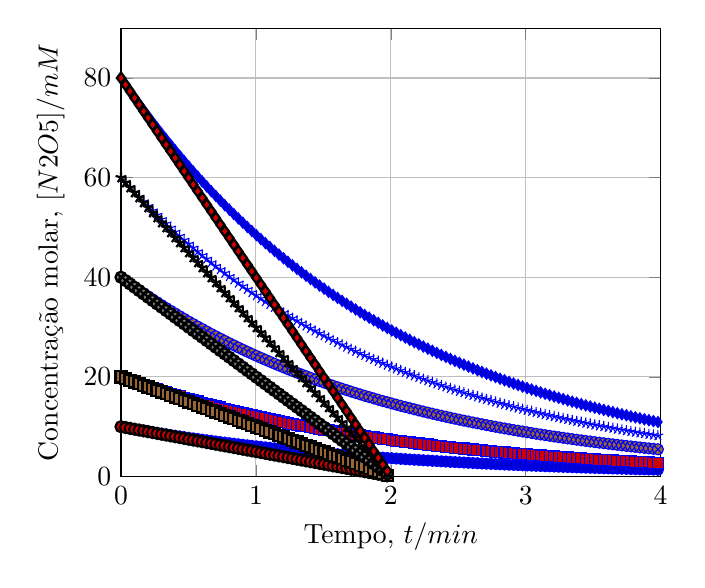
\begin{tikzpicture}
    \begin{axis}
        [
            xlabel = {Tempo, $t/\unit{min}$},
            ylabel = {Concentração molar, $[\ce{N2O5}]/\unit{mM}$},
            ymin = 0, ymax = 90,
            xmin = 0, xmax = 4,
            domain = 0:10,
            grid = major,
            samples = 300,
        ]
    
    \addplot+ [blue]
        {
            10 * e^(-x/2)
        };

    \addplot+ [blue]
        {
            20 * e^(-x/2)
        };

    \addplot+ [blue]
        {
            40 * e^(-x/2)
        };

    \addplot+ [blue]
        {
            60 * e^(-x/2)
        };
    
    \addplot+ [blue]
        {
            80 * e^(-x/2)
        };
        
     \addplot+ [black, thick]
        {
            10*(1 - x/2)
        };
    
    \addplot+ [black, thick]
        {
            20*(1 - x/2)
        };
    
    \addplot+ [black, thick]
        {
            40*(1 - x/2)
        };
    
    \addplot+ [black, thick]
        {
            60*(1 - x/2)
        };
    
    \addplot+ [black, thick]
        {
            80*(1 - x/2)
        };

    \end{axis}
\end{tikzpicture}